\documentclass[fontsize=12pt]{scrartcl}
\usepackage[ngerman]{babel}
\usepackage[utf8]{inputenc}
%\usepackage[latin1]{inputenc}
\usepackage{amsmath}
\usepackage{amstext}
\usepackage{amssymb}
\usepackage{stmaryrd}
\usepackage{verbatim}
\usepackage{mathrsfs}
\usepackage{extarrows}
\usepackage[arrow, matrix, curve]{xy}
\usepackage[centering,includeheadfoot,margin=2cm]{geometry}
\usepackage{gensymb}
\usepackage{graphicx}
\usepackage{framed}
\usepackage{xcolor}
\usepackage{float}
\usepackage{graphicx} 
\usepackage{sidecap}
\usepackage{blindtext,wrapfig}
\usepackage{epstopdf}
\usepackage{import}
\usepackage{fancyhdr}
\usepackage{fancybox}
\usepackage{paralist}
\usepackage{graphicx}
\usepackage{caption}
\usepackage{subcaption}
\renewcommand{\l}{\left\vert}
\renewcommand{\r}{\right\vert}
\DeclareGraphicsRule{.tif}{png}{.png}{`convert #1 `basename #1 .tif`.png} 
\pagestyle{fancy}
\fancyhf{}
\fancyhead[R]{Physikalisches Praktikum 1}
\fancyhead[L]{Linda Werneck, Gentian Rrafshi}
\fancyfoot[R]{\thepage}
\fancyfoot[L]{\today}

\begin{document}

\begin{minipage}{\textwidth}
\begin{center}\large
\title{ E24b – Halbleiterdioden \\
		~\\
		~\\
		Assistent: Niklas Liebermann \\
		Datum Versuchsdurchführung: \\
		17.06.2015}

\author{bearbeitet von\\
		Gruppe 3-031: \\
		Linda Werneck Matrnr. 2901495 \\
		Gentian Rrafshi Matrnr. 2721617 }
\date{\today}

\maketitle

\end{center}
\end{minipage}

\newpage

\tableofcontents

\newpage
\noindent

\section{ Versuchsziel}
Ziel des Versuchs ist Messreihen zu den Durchlass- und Sperrrichtkennlinien von jeweils einer Germanium-, Silizium-, Zener- und Leuchtdiode zu erhalten um 
den Sperrstrom zu berechnen.

\section{ Grundlagen}

Betrachten wir einen Ladungsträger, so sind sowohl das elektrische Feld $E(x)$ und die Dichten ortsabhängig. Man kann nun die Löcherdichten $p(x)$ oder
die Elektronendichten $n(x)$ betrachten. Ohne Beschränkung nehmen schauen wir uns hier die Löcherdichten an, da die Rechnung für die Elektronendichten 
analog verläuft. Betrachtet man nun auf dem Ladungsträger den Feldstrom, so weiß man, dass der Feldstrom proportional zum Feld, der Löcherdichte, zu deren Beweglichkeit $\nu$ und der Ladung $q$. Wir können ohne Einschränkung annehmen, dass die Beweglichkeit $\nu$ nicht vom Feld abhängt und erhalten damit für den Feldstrom:
\begin{equation}
j_{\text{Feld}}= q \cdot \nu \cdot p(x) \cdot E(x)
\end{equation}
Aufgrund der Tatsache, dass Ladungsträger vom orten hoher Konzentration zu niedriger Konzentration sich bewegen, erhalten wir beim Diffusionsstrom, dass er sich entgegen dem Gradienten der Ladungsträgerkonzentration bewegt. Daher erhalten wir für den Diffusionsstrom:
\begin{equation}
j_{\text{Diff}}= - q \cdot D\cdot \frac{\partial p(x)}{\partial x}
\end{equation}
Wobei D eine Diffusionskonstante beschreibt, welche die Stärke der Diffusion darstellen soll.\\
~\\
Schaut man sich nun den stationären Fall  $j_{\text{Feld}}=j_{\text{Diff}}$ an, so ergibt sich:
\begin{align*}
q \cdot \nu \cdot p(x) \cdot E(x) &=- q \cdot D\cdot \frac{\partial p(x)}{\partial x} \\
\frac{\nu}{D}\cdot E(x) &= \frac{1}{p(x)}\cdot \frac{\partial p(x)}{\partial x}  \qquad\qquad \mid\text{Einstein-Beziehung} \frac{D}{\nu}=\frac{kT}{q}\\
\frac{-q}{kT} \frac{\partial U(x)}{\partial x} &=  \frac{1}{p(x)}\cdot \frac{\partial p(x)}{\partial x} \qquad\qquad\mid \cdot \partial x\\
\frac{-q}{kT} \partial U(x) &=  \frac{ \partial p(x)}{p(x)} \\
\frac{-q}{kT} \int^{U_n}_{U_p}  \partial U(x)  &=  \int^{p_n}_{p_p}  \frac{ \partial p(x)}{p(x)} \\
\frac{-q}{kT} (U_n-U_p) &= \ln\left(\frac{ p_n}{p_p}\right) \qquad\qquad\qquad \mid U = U_n-U_p	 \\
\frac{q\cdot U}{kT}  &= \ln\left(\frac{ p_p}{p_n}\right) \qquad\qquad\qquad \mid e^{\bullet} \\
p_p &=  p_n \cdot e^{\frac{q\cdot U}{kT} }
\end{align*}
\newpage
\noindent
Was wir nun anschauen ist $\Delta p = p_p-p_{n}$, wobei $p_{n}$ und $p_p$ die Löcherdichten kurz außerhalb der Grenzschicht im $n$- und $p$-Bereich sind. Damit ist dann $\Delta p$ die dazugewonnen Löcherdichte, wobei mit dem Gleichgewichtszustand verglichen wird. Dann erhalten wir:
\begin{equation}
\Delta p = p_n \cdot (e^{\frac{q\cdot U}{kT} } - 1)
\end{equation}
Da nun die Löcherdichte und  die Stromstärke proportional zueinander sind, ergibt sich für $\Delta p = I$ und $p_n = I_S$:
\begin{equation}
I=I_S\cdot[e^{\frac{e\cdot U}{kT}}-1]
\end{equation}
\noindent
Was die sogenannte Shockleysche Beziehung ist. 
\section{Versuchsaufbau und Durchführung}

\subsection{benötigte Geräte}

Um den Versuch durchführen zu können benötigt man:
\begin{itemize}
\item	Germanium-, Silizium-, Zener-Diode
\item	blau und rot leuchtende LEDs
\item	Steckbrett mit Widerständen
\item	Frequenzgenerator
\item	Gleichstromgenerator
\item	Strom und Spannungsmessgerät
\item	Kabel
\item	Oszilloskop
\end{itemize}

\subsection{Messungen mit Gleichstrom}
Der Versuchsablauf für die Zener-, Silizium- und Germaniumdiode ist gleich. Im Folgenden wird der Versuchsablauf an der Silizium-Diode erläutert, die 
Messungen an den zwei anderen Dioden sind analog dazu durchzuführen. 
\begin{figure}[h!]
\centering
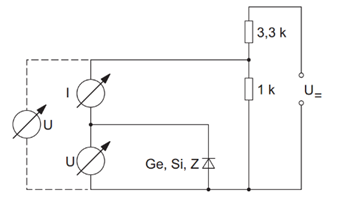
\includegraphics[scale=1]{Graphik/Versuch1}
\caption{Versuchsskizze$^{\cite{A}}$}
\label{1}
\end{figure}\\
An der Silizium-Diode wird mit Gleichstrom gearbeitet. Zunächst wird der Versuch wie in Abbildung \ref{1} Aufgebaut. Die Messanordnung ist so eingestellt, 
dass man in Durchlassrichtung misst. Dazu stellt man die Spannung so ein, dass der Strom einen gewünschten Wert erreicht. Der erste Zielwert liegt bei 0,05 
mA. Die dazugehörige eingestellte Spannung wird notiert. Der nächste Zielwert, der eingestellt werden muss, liegt bei 0,1 mA und so erhöhen sich die 
Zielwerte immer um einen Faktor zwei. \\
\noindent
Die zu den Stromstärken gehörenden Spannungen werden immer notiert. Das Steckbrett wirdumgebaut. Die Kathode und Anode werden vertauscht, sodass 
man in Sperrrichtung misst. Nun beginnt die Messung bei einer Spannung von 1 V, die Stromstärke wird abgelesen und notiert. Der nächste Messwert liegt 
bei 2 V. Die Spannung wird so immer um 1 V bis zu ca. 7 V erhöht, die dazugehörigen Stromstärken werden notiert.
Die Messungen an der Silizium-Diode sind damit beendet.

\subsection{Messungen mit Wechselstrom}
 \begin{figure}[h!]
\centering
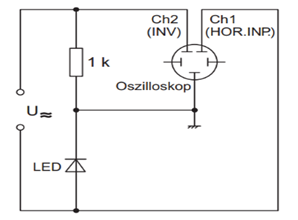
\includegraphics[scale=1]{Graphik/Versuch2}
\caption{Versuchsskizze$^{\cite{A}}$}
\label{2}
\end{figure}
\noindent
Die Messungen an der roten und blauen Leuchtdiode werden mit Wechselstrom gemacht und sind analog zueinander durchzuführen. Der Versuch wird wie in 
Abbildung \ref{2} aufgebaut. Auf dem Oszilloskop wird das „Format XY“ eingestellt und der Kanal 2 wird invertiert. Man erhält darauf hin übliche 
Kennliniendarstellung für die LEDs. Diese wird fotografiert.

\newpage


\section{Formeln}

\subsection{Shockleysche Beziehung} 

\begin{equation}
I=I_S\cdot[e^{\frac{e\cdot U}{kT}}-1]
\end{equation}
$I$: Strom, $U$: Spannung, $I_S$: Sperrstrom, $e$: Elementarladung, $k$: Bolzmankonstante, \\
$T$: absolute Temperatur

\subsection{Energie eines Lichtteilchens}

\begin{equation}
E_{\text{Licht}}=h\cdot \nu =\frac{h\cdot c}{\lambda}
\label{E}
\end{equation}
$h$: Plancksches Wirkungsquantum, $c$: Lichtgeschwindigkeit, $\lambda$ : Wellenlänge; $\nu$ Frequenz


\newpage

\section{ Messwerte}
\begin{figure}[H]
\caption{Messwerte für Germaniumdiode}
\begin{minipage}{0.5\textwidth}
\vspace{-15pt}
\centering
\begin{tabular}{|c|c|} \hline
\multicolumn{2}{|c|}{ Sperrrichtung	}\\ \hline
Spannung in [V]	& Strom in  [$\mu$A] \\ \hline
-1,00	&-0,40\\ \hline
-2,00	&-0,50\\ \hline
-3,00	&-0,70\\ \hline
-4,00	&-0,80\\ \hline
-5,00	&-1,00\\ \hline
-6,00	&-1,10\\ \hline
-7,00	&-1,30\\ \hline
-7,30	&-1,40\\ \hline
\end{tabular} \\
\end{minipage}
\begin{minipage}{0.2\textwidth}
\centering
\begin{tabular}{|c|c|} \hline
\multicolumn{2}{|c|}{ Durchlassrichtung}	\\ \hline
Spannung in [V]	& Strom in  [mA] \\ \hline
0,1450	&0,05\\ \hline
0,1680	&0,10\\ \hline
0,2000	&0,20\\ \hline
0,2280	&0,40\\ \hline
0,2600	&0,80\\ \hline
0,2950	&1,60\\ \hline
0,3350	&3,20\\ \hline
0,3850	&6,40\\ \hline
0,4110	&8,90\\ \hline
\end{tabular} \\
\end{minipage}
\end{figure}
\vspace{-20pt}
\begin{figure}[H]
\caption{Messwerte für Siliziumdiode}
\begin{minipage}{0.5\textwidth}
\vspace{-15pt}
\centering
\begin{tabular}{|c|c|} \hline
\multicolumn{2}{|c|}{ Sperrrichtung	}\\ \hline
Spannung in [V]	& Strom in  [$\mu$A] \\ \hline
-1,00	&-0,20\\ \hline
-2,00	&-0,30\\ \hline
-3,00 	&-0,40\\ \hline
-4,00	&-0,50\\ \hline
-5,00	&-0,60\\ \hline
-6,00	&-0,70\\ \hline
-7,00	&-0,80\\ \hline
-7,30	&-0,83\\ \hline
\end{tabular} \\
\end{minipage}
\begin{minipage}{0.2\textwidth}
\centering
\begin{tabular}{|c|c|} \hline
\multicolumn{2}{|c|}{ Durchlassrichtung}	\\ \hline
Spannung in [V]	& Strom in  [mA] \\ \hline
0,46	&0,05\\ \hline
0,50	&0,10\\ \hline
0,53	&0,20\\ \hline
0,57	&0,40\\ \hline
0,61	&0,80\\ \hline
0,64	&1,60\\ \hline
0,69	&3,20\\ \hline
0,73	&6,40\\ \hline
0,75	&8,50\\ \hline
\end{tabular} \\
\end{minipage}
\end{figure}
\vspace{-20pt}	
\begin{figure}[H]
\caption{Messwerte für Zenerdiode}
\begin{minipage}{0.5\textwidth}
\vspace{-15pt}
\centering
\begin{tabular}{|c|c|} \hline
\multicolumn{2}{|c|}{ Sperrrichtung	}\\ \hline
Spannung in [V]	& Strom in  [mA] \\ \hline
-1,00	&-0,20\\ \hline
-2,00	&-0,30\\ \hline
-3,00	&-0,70\\ \hline
-4,00	&-11,20\\ \hline
-5,00	&-168,00\\ \hline
-5,30	&-1485,00\\ \hline
\end{tabular} \\
\end{minipage}
\begin{minipage}{0.2\textwidth}
\centering
\begin{tabular}{|c|c|} \hline
\multicolumn{2}{|c|}{ Durchlassrichtung}	\\ \hline
Spannung in [V]	& Strom in  [mA] \\ \hline
0,6200&	0,05\\ \hline
0,6500&	0,10\\ \hline
0,6700&	0,20\\ \hline
0,7000&	0,40\\ \hline
0,7100&	0,80\\ \hline
0,7300&	1,60\\ \hline
0,7600&	3,20\\ \hline
0,7800&	6,40\\ \hline
0,7970&	8,35\\ \hline
\end{tabular} \\
\end{minipage}\\
\end{figure}

\newpage

\section{ Auswertung}

\subsection{Germanium- und Silizium-Diode}

Im ersten Teil des Versuchs sollen wir ein Strom-Spannung-Diagramm für in Sperr- und Durchlassrichtung für jeweils die Germanium- und Silizium-Diode erstellen. Zuerst die Durchlassrichtung:\\
\begin{figure}[H]
\vspace{-20pt}
\centering
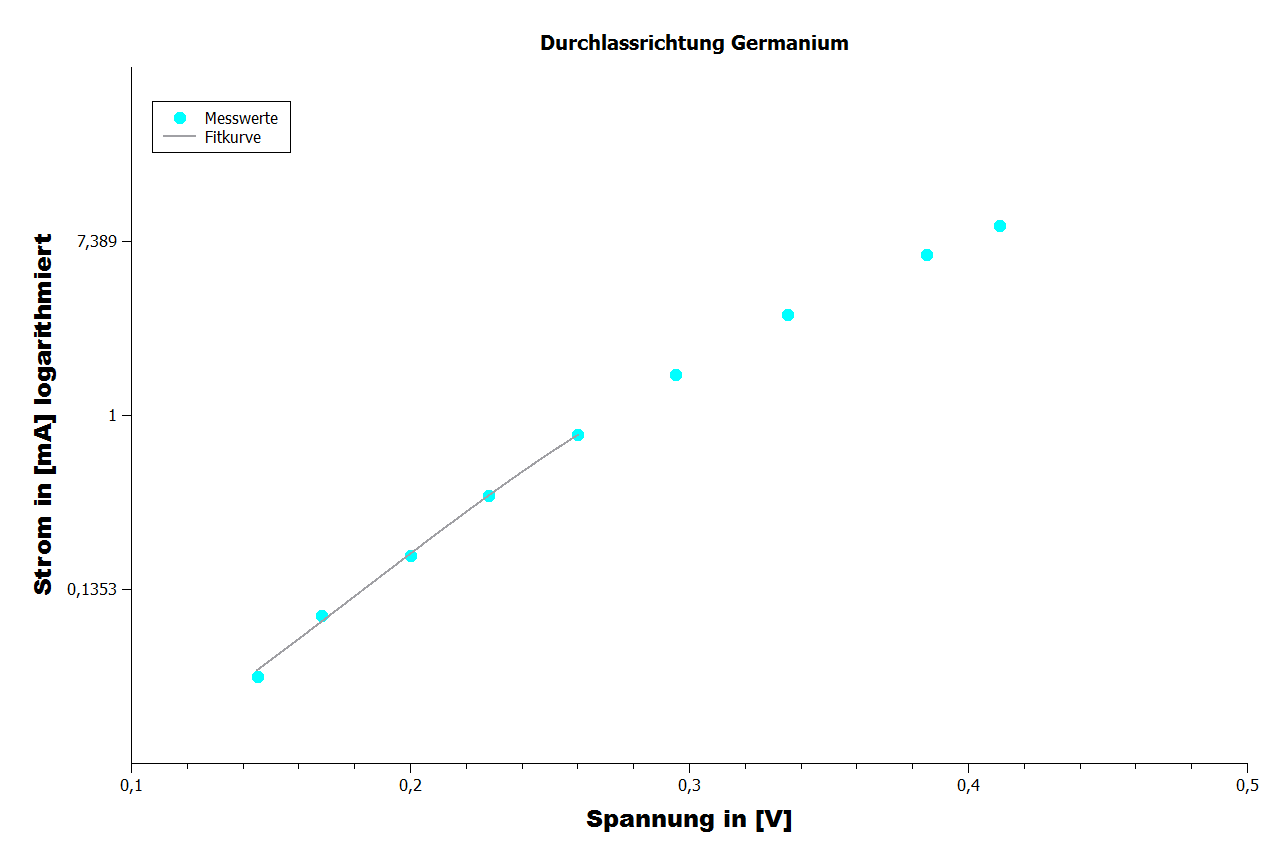
\includegraphics[scale=0.35]{Graphik/Germanium_Durchlass}
\caption{Germanium-Diode in Durchlassrichtung}
\end{figure}
\noindent
\begin{figure}[H]
\vspace{-20pt}
\centering
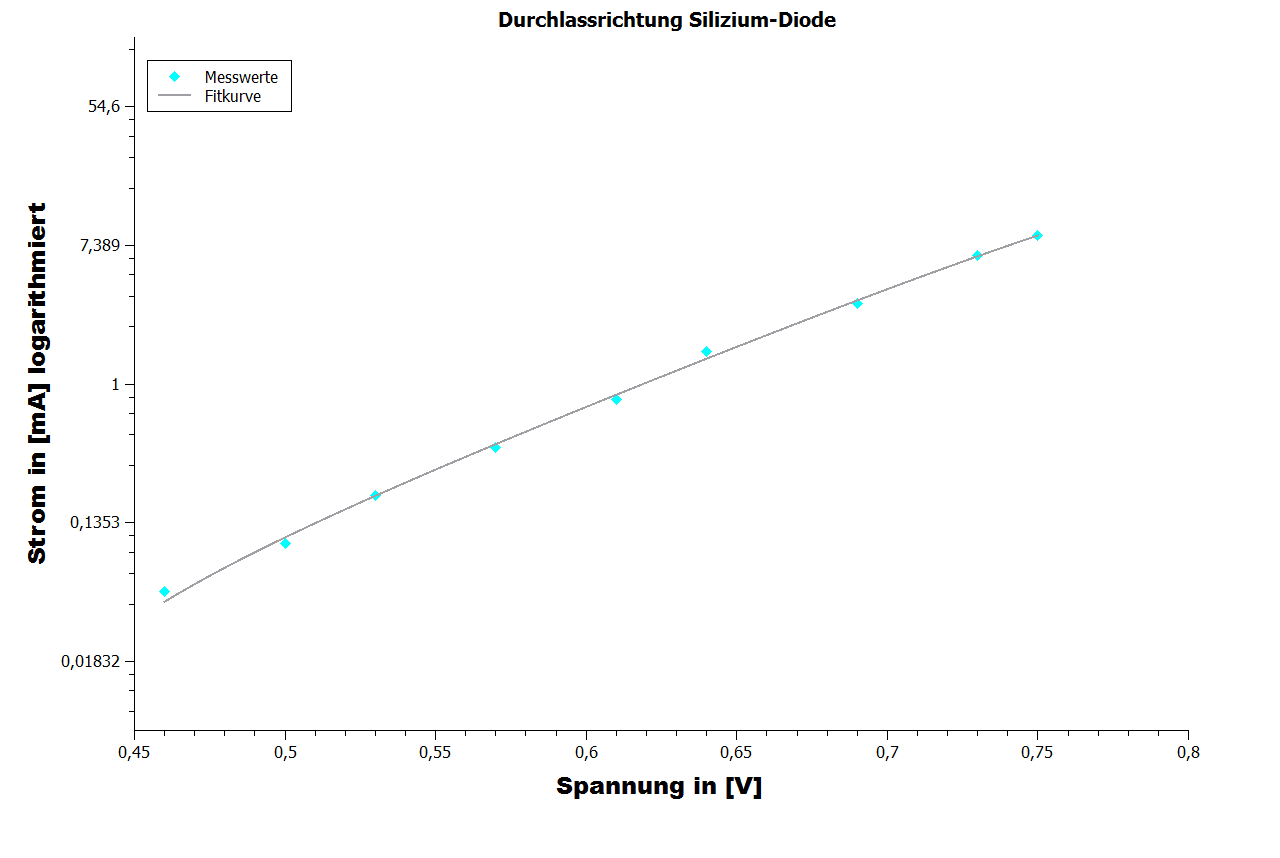
\includegraphics[scale=0.35]{Graphik/Silizium_Durchlass}
\caption{Silizium-Diode in Durchlassrichtung}
\end{figure}
\newpage
\noindent
Ein Ziel dieses Versuchs ist es, den Sperrstrom $I_S$ zu bestimmen, dazu haben wir an unsere Messwerte jeweils eine Exponentialfunktion gefittet und durch Extrapolation zu $U=0$\,V erhalten wir folgende Werte für den Sperrstrom:
\begin{itemize}
\item Für Germanium erhalten wir für den Sperrstrom $I_S=0,006\,mA$
\item Für Silizium erhalten wir für den Sperrstrom $I_S=0,020\,mA$
\end{itemize}
\noindent
~\\
Nun kommen die linearen Plots für die Sperrrichtung:\\
\begin{figure}[H]
\centering
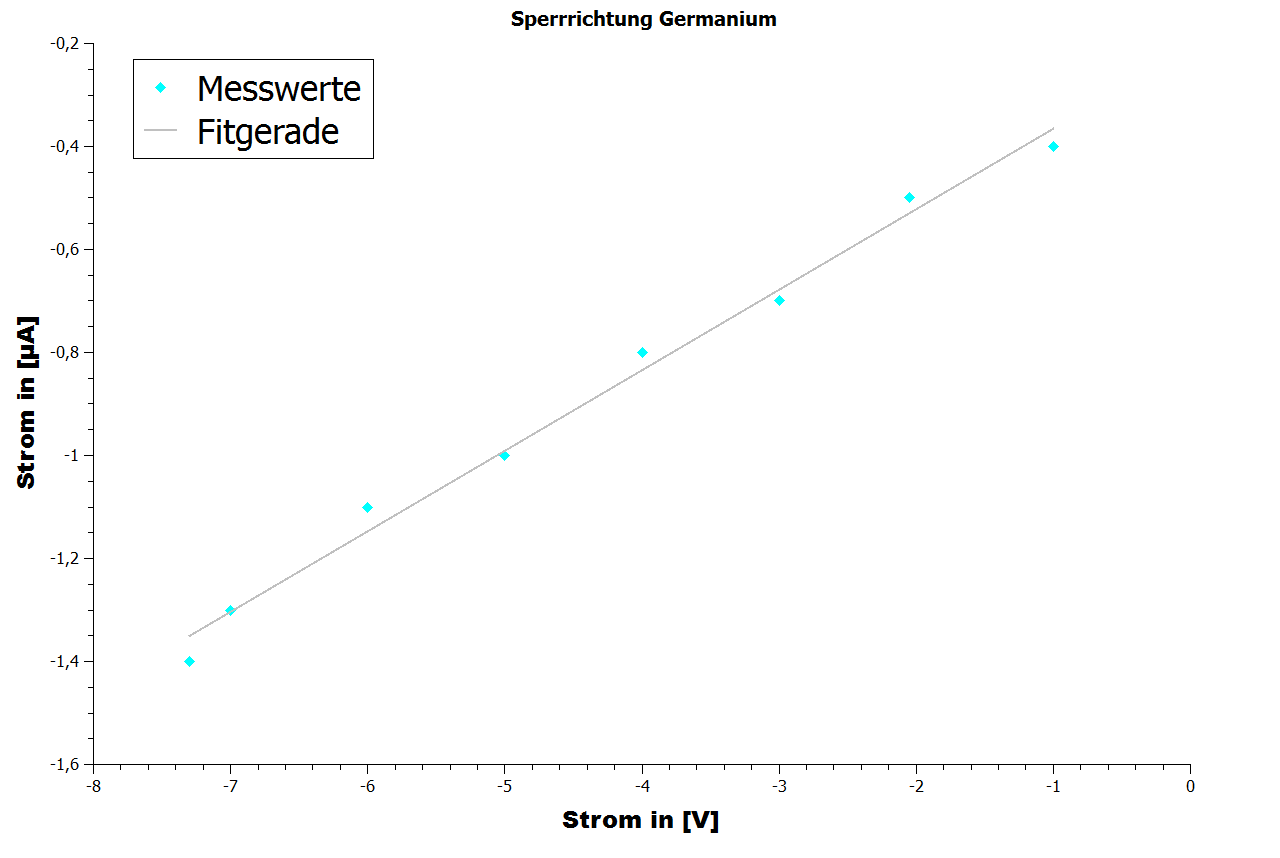
\includegraphics[scale=0.4]{Graphik/Germanium_Sperr}
\caption{Germanium-Diode in Sperrrichtung}
\end{figure}
\noindent
\begin{figure}[H]
\centering
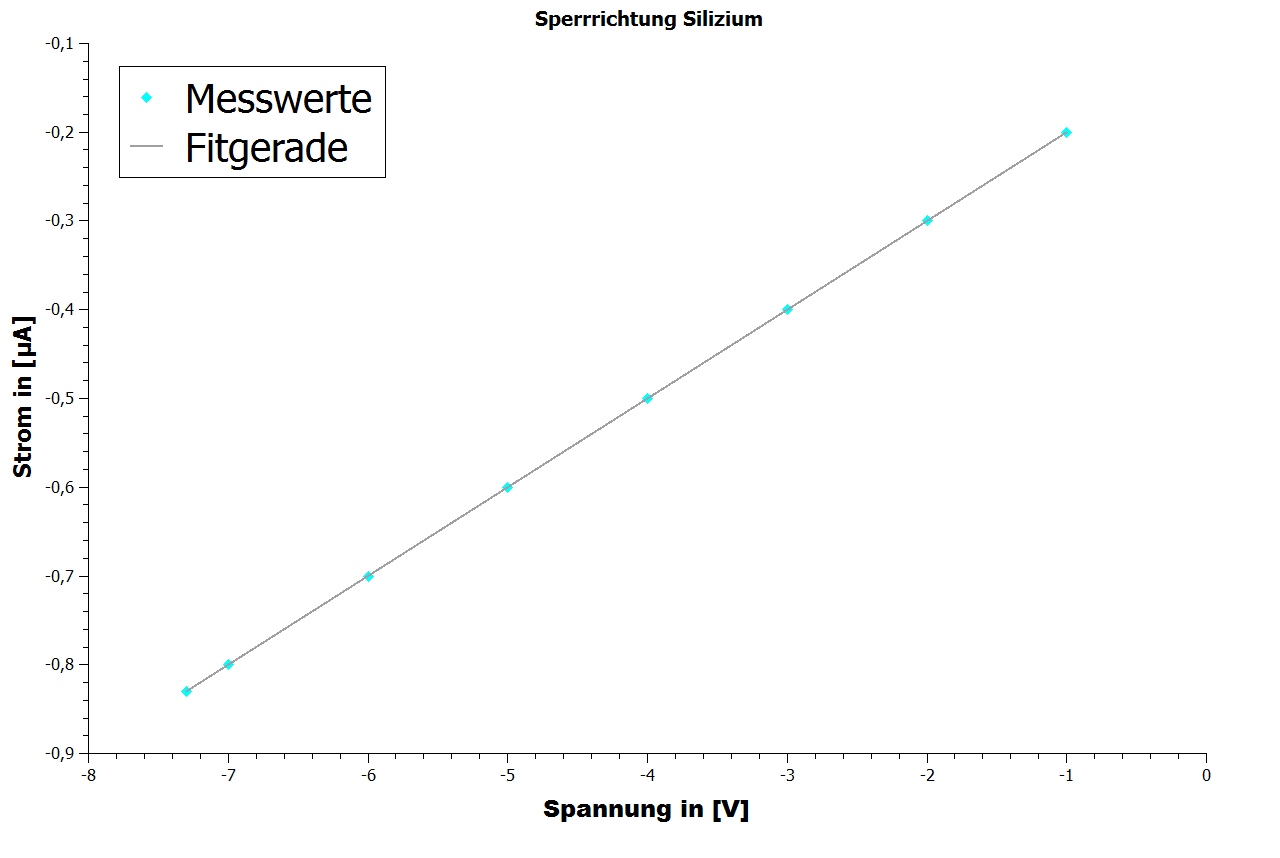
\includegraphics[scale=0.4]{Graphik/Silizium_Sperr}
\caption{Silizium-Diode in Sperrrichtung}
\end{figure}


\newpage

\subsection{Zener-Diode}

Für die Zenerdiode sollen wir ein lineares Diagramm erstellen, indem der Zusammenhang zwischen Strom und Spannung ersichtlich werden soll. wir erhalten mit unseren Messwerten folgendes Diagramm:\\
\begin{figure}[H]
\vspace{-20pt}
\centering
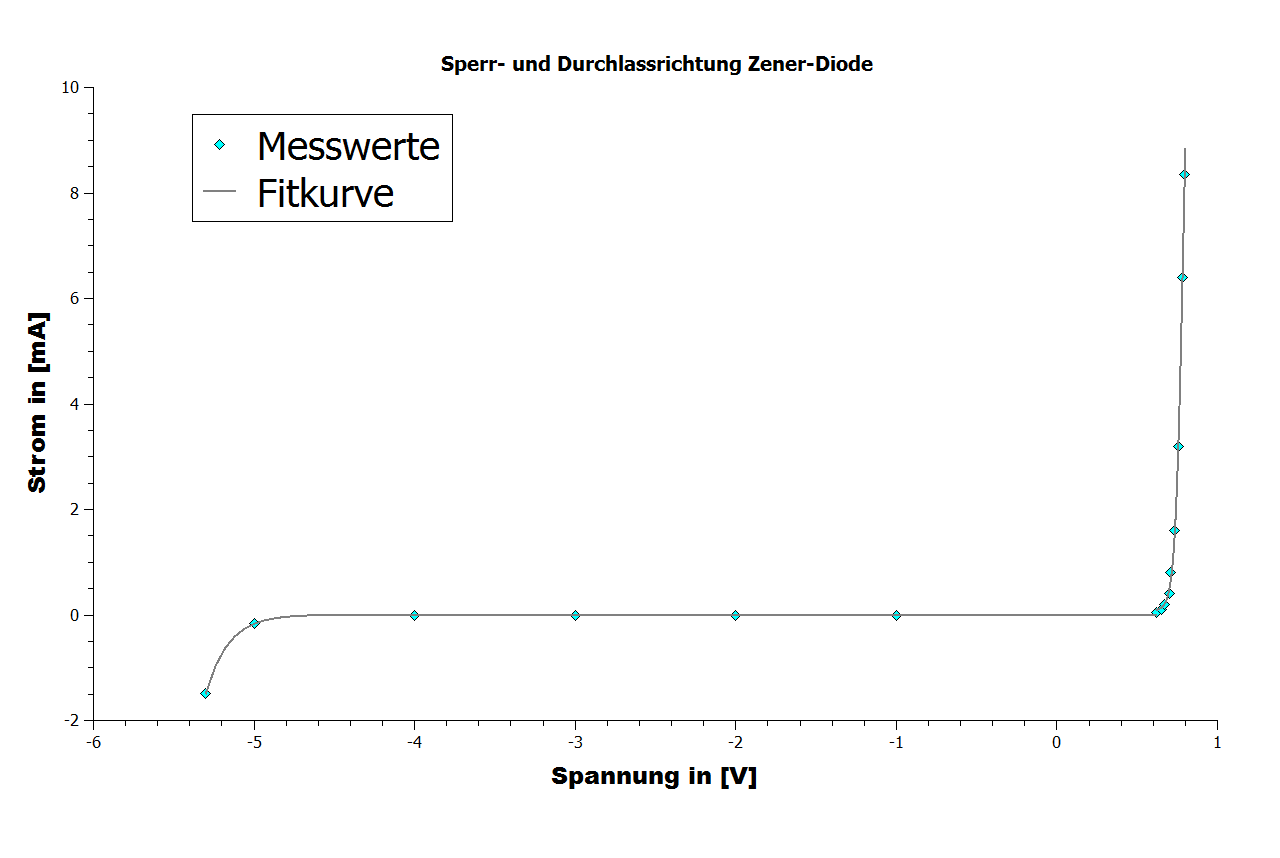
\includegraphics[scale=0.35]{Graphik/Zener}
\caption{Zener-Diode in Sperr- und Durchlassrichtung}
\end{figure}
\noindent
Da man in Durchlassrichtung so gut wie gar nicht die Messwerte erkennt, 
wird hier nochmals jeweils ein Diagramm für Sperr- und Durchlassrichtung eingefügt:\\
\begin{figure}[H]
\vspace{-20pt}
\centering
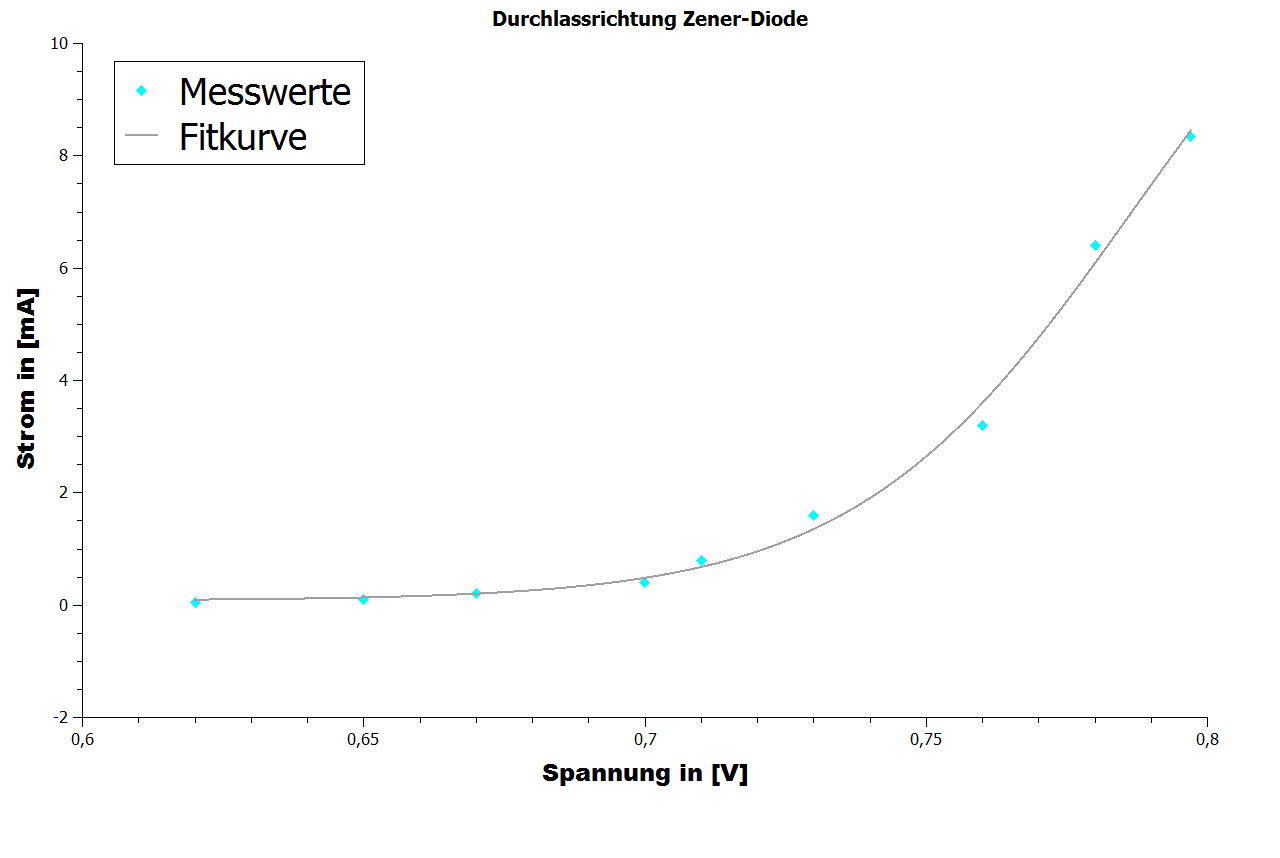
\includegraphics[scale=0.35]{Graphik/Zener_Durchlass}
\caption{Zener-Diode in Durchlassrichtung}
\end{figure}
\noindent
\begin{figure}[H]
\centering
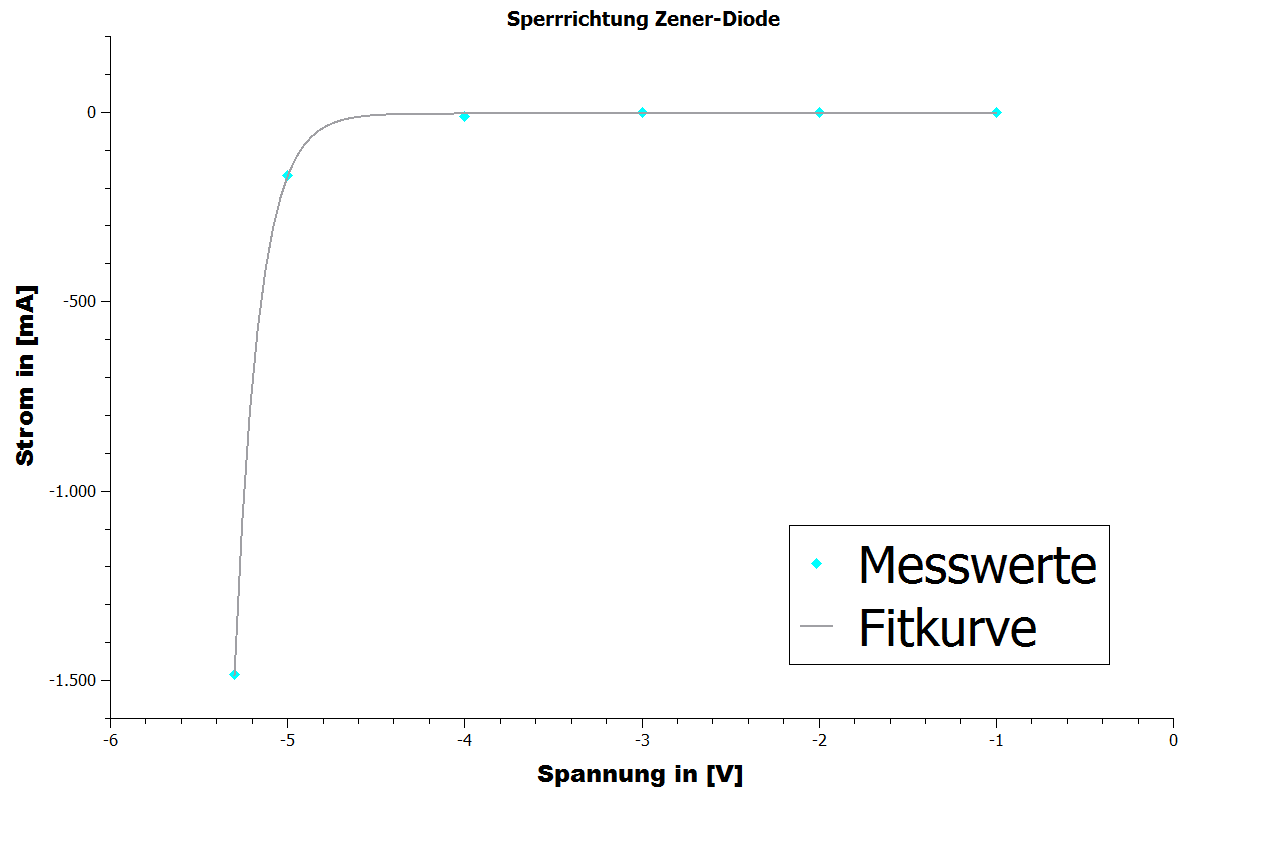
\includegraphics[scale=0.35]{Graphik/Zener_Sperr}
\caption{Zener-Diode in Sperrrichtung}
\label{3}
\end{figure}
\noindent
An Diagramm (\ref{3}) erkennt nochmal schön, dass ab eine Spannung von $\approx 4,8$\,V die Zenerdiode durchbricht.
\newpage

\subsection{LEDs}

In diesem letzten Teil des Versuchs sollten wir die Kennlinien von einer roten und blauen Leuchtdiode bestimmen. An den folgenden Bildern sieht man jeweils unten die Schwellspannung. Diese beträgt bei uns für die rote LED eine Schwellspannung von $U_S=1,74$\,V und bei der blauen $U_S=2,56$\,V.

\begin{figure}[H]
\centering
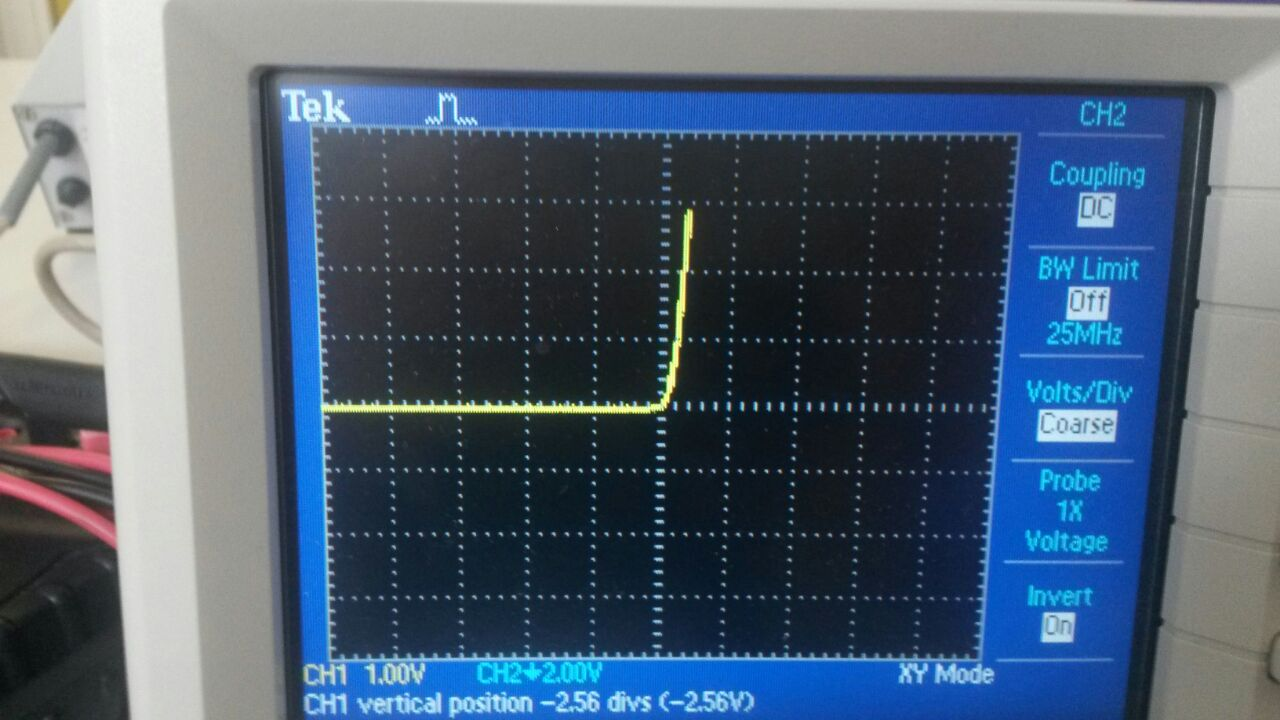
\includegraphics[scale=0.2]{Graphik/blau1}
\caption{Kennlinie blaue LED}
\end{figure}
\noindent
\begin{figure}[H]
\vspace{-20pt}
\centering
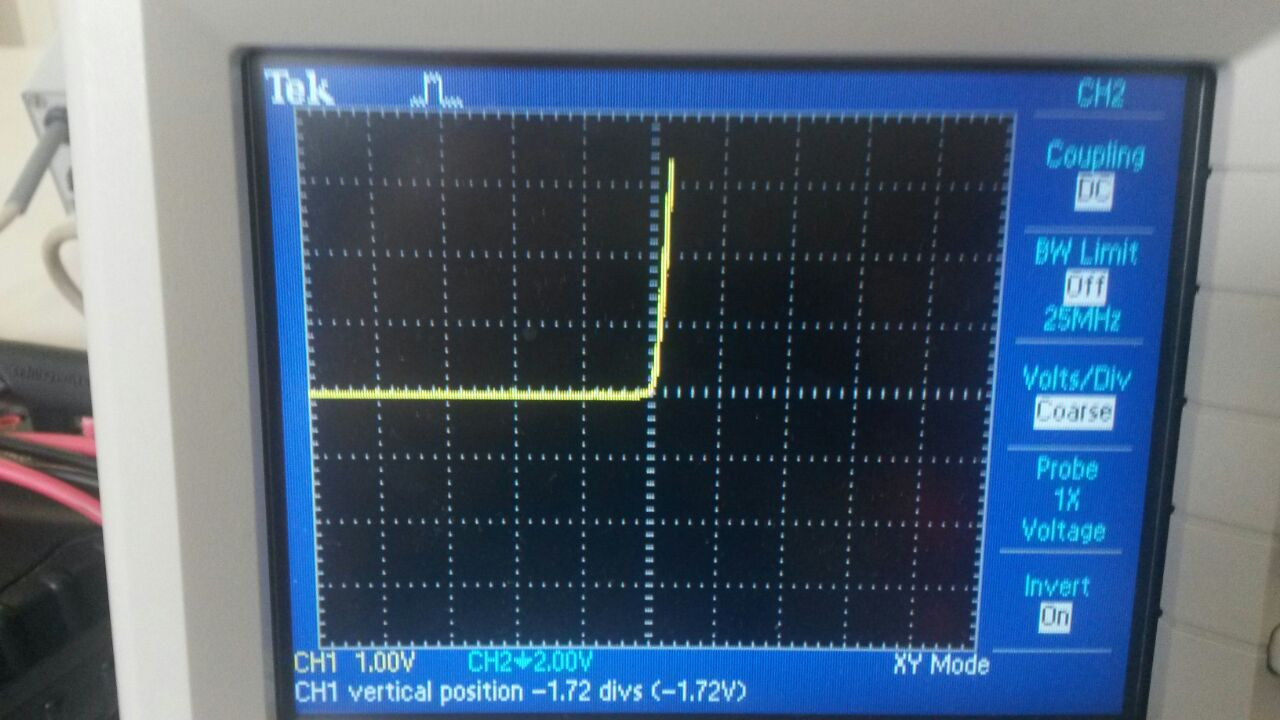
\includegraphics[scale=0.2]{Graphik/rot1}
\caption{Kennlinie rote LED}
\end{figure}
\noindent
Setzen wir Formel (\ref{E}) mit der kinetischen Energie $E_{\text{kin}}=eU$ von Elektronen gleich, so erhalten wir folgende Proportion:
\begin{align*}
U \propto \frac{1}{\lambda}
\end{align*}
Da rotes Licht eine Wellenlänge von  $790–630$\,nm und blaues Licht etwa $480–420$\,nm als Wellenlänge hat, stimmen unsere Messungen mit der Proportionalität über ein, da das rote Licht mit der große Wellenlänge die niedrigere Schwellspannung hat und blaues Licht eine höhere Schwellspannung hat.
\newpage
\noindent
Desweiteren ergibt sich durch gleichsetzen folgende Formel für die Schwellspannung:
\begin{align*}
U=\frac{h\cdot c}{e\cdot \lambda} &=\frac{6,626 069 57 \cdot 10^{-34}\,\text{Js} \cdot 299792458\,\frac{\text{m}}{\text{s}}}
{1,602\cdot 10^{-19}\,\text{C}\cdot \lambda}\\
&=\frac{1,2415155\cdot 10^{12}\text{Vm}}{\lambda}
\end{align*}
Wir haben nun jeweils eine Spannung für beide LED`s und können damit zurückrechnen, was für eine Wellenlänge unsere Dioden haben sollten:\\
\begin{align*}
\lambda_{S_{rot}}&=\frac{1,2415155\cdot 10^{12}\text{Vm}}{1,74\,\text{V}}=7,2141\cdot10^{-7}\,\text{m}=721,41\,\text{nm}\\
\lambda_{S_{blau}}&=\frac{1,2415155\cdot 10^{12}\text{Vm}}{2,56\,\text{V}}=4,8470\cdot10^{-7}\,\text{m}=484,70\,\text{nm}
\end{align*}
Unsere gemessen Werte ergeben also Wellenlänge, die im Bereich von roten bzw. blauen Licht liegen.

\subsection{Fragen}

Eine weitere Aufgabe ist es, die Funktion der Widerstände in Abbildung (\ref{1}) und die Funktionsweise der Schaltung in Abbildung (\ref{2}) zu beschreiben:\\
~\\
\textbf{zu Abbildung (\ref{1})}:\\
Der 3,3 k$\Omega$ Widerstand schützt die jeweilige Diode vor zu hohen Strömen in Durchlassrichtung, während in Sperrrichtung der 1 k$\Omega$ Widerstand die jeweilige Diode stützt.\\
~\\
\textbf{zu Abbildung (\ref{2})}:\\
Wichtig ist es zu wissen, dass nur die positive Halbwelle, d.h. die Halbwelle an der bei der Anode positive Spannung anliegt, überhaupt durchgelassen wird. Ab dem Zeitpunkt, an dem die Schwellspannung erreicht beziehungsweise überschritten wird, beginnt dann die LED zu leuchten.  \\
~\\
Am Kanal 2 muss das Eingangssignal schaltungsbedingt invertiert werden. Erreicht eine negative Halbwelle die LED, so sperrt die LED und hat einen sehr großen Widerstand, d.h. die LED wird hochohmig. Daher fängt der Widerstand dann die gesamte anliegende Spannung ab, wenn er richtig herum eingebaut wurde. Im Falle der positiven Halbwelle ist es umgekehrt,d.h. die LED besitzt einen geringen ohmschen Widerstand.
Der Widerstand wird gebraucht, damit am Oszilloskop eine Spannung abfällt. Damit sind dann die Diodenkennlinien erst Darstellbar.  
\newpage

\section{Zusammenfassung}

Für diesen Versuch sollten wir die Diodenkennlinien verschiedener Dioden, unter anderem zwei LEDs, bestimmen. 
Wir fanden im ersten Teil des Versuchs, dass Germanium-Dioden eine kleinere Diffusionsspannung in Durchlassrichtung haben und man daher diese besser nutzen kann, wenn man mit kleinen Spannungen arbeiten möchte. Der Nachteil der Germanium-Diode ist aber, dass in Sperrrichtung kaum Spannung sperren. Dafür ist die Silizium-Diode geeigneter, da sie im Vergleich zu Germanium-Dioden eine höher Sperrspannung hat. \\
~\\
Schön ersichtlich wird es an diesem Diagramm, welches die Kennlinien für Ströme bis zu 100\,mA in Durchlassrichtung bzw. 50\,$\mu$A in Sperrrichtung 
anzeigt:
\begin{figure}[H]
\centering
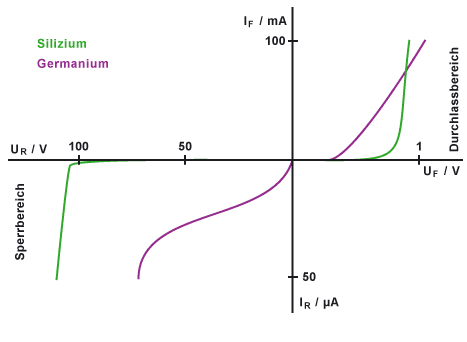
\includegraphics[scale=1]{Graphik/bsp}
\caption{Kennlinien für Germanium und Silizium-Dioden$^{\cite{B}}$}
\end{figure}
\noindent
Auch zu sehen ist, dass bei Silizium kleine Spannungsänderungen in Durchlassrichtung schnell hohe Stromänderung zu folge hat, was bei Germanium ab einem gewissen Zeitpunkt quasi linear Änderung ergibt. Wir haben durch Extrapolation folgende Sperrströme bekommen:
\begin{itemize}
\item Für Germanium erhalten wir für den Sperrstrom $I_S=0,006\,mA$
\item Für Silizium erhalten wir für den Sperrstrom $I_S=0,020\,mA$
\end{itemize}
\noindent
Im zweiten Teil sehen wir, dass die Zener-Diode eine stark dotierte Silizium-Diode ist, was erklärt warum bei kleinen Spannung schon größerer Ströme 
entstehen. Ein Vorteil der Zener-Diode ist, dass bei Sperrspannung nicht zur Zerstörung der Diode kommt und die Diode leitet ab der Sperrspannung 
Strom sehr gut.\\
\newpage
\noindent
Im Letzten Teil des Versuchs ging es um LEDs, speziell eine rote leuchtende LED und blau leuchtende. Durch Gleichsetzen von  $E_{\text{kin}}=E_{\text{Licht}}$ erhält man eine Proportionalität zwischen der Spannungsschwelle und Wellenlänge, die wie folgt aussieht:
\begin{align*}
U \propto \frac{1}{\lambda}
\end{align*}
Diese Proportionalität haben wir bei unseren Messungen auch gesehen. Für uns ergaben sich folgende Werte für die Spannungsschwelle:
\begin{figure}[H]
\vspace{-15pt}
\caption{Spannungsschwellen bei LEDs}
\centering
\begin{tabular}{|l|c|c|} \hline
\multicolumn{3}{|c|}{ Spannungsschwelle}\\ \hline
LED &gemessen [V]	& errechnet  [V] \\ \hline
rote LED		& 1,72	& 1,75\\ \hline
blaue LED	& 2,56	& 2,75\\ \hline
\end{tabular} \\
\end{figure}


\newpage
\section{Literaturverzeichnis}

\renewcommand{\refname}{~}
\vspace{-30pt}
\begin{thebibliography}{xx}
	\bibitem[1]{1}		\textit{\glqq E24 Halbleiterdioden\grqq , \\
								 in http:www3.physik.uni-stuttgart.de/studium/praktika/ap/},\\
								unter \textit{http://www3.physik.uni-stuttgart.de/studium/praktika/ap/pdf\_dateien/E24.pdf}; \\
								 abgerufen am 20.06.2015
   \bibitem[A]{A}  	Graphik aus \textit{\glqq E24 Halbleiterdioden\grqq , in 	\\
   								http://www3.physik.uni-stuttgart.de/studium/praktika/ap/}, \\
   								unter \textit{http://www3.physik.uni-stuttgart.de/studium/praktika/ap/pdf\_dateien/E24.pdf}; \\
   								abgerufen am 20.06.2015 
   \bibitem[B]{B}  	Graphik aus \textit{http://www.elektronik-kompendium.de/sites/bau/diagramm/02011131.gif}, \\
   								abgerufen am 20.06.2015
\end{thebibliography}

\section{Anhang}

\end{document}